\documentclass[a4paper, 12pt, titlepage]{article}
\usepackage[utf8]{inputenc}
\usepackage{geometry}
\usepackage{polski}
\usepackage{graphicx}
\usepackage{float}
\usepackage{etoolbox,refcount}
\usepackage{multicol}
\usepackage{fancyhdr}
\usepackage{caption}
%\pagestyle{fancy}
\title{Projekt i realizacja tensometrycznych przetworników pomiarowych siły i massy z wykorzystaniem belki giętej i przemysłowego panelu wzmacniacza tensometrycznego MVD555}
\author{\textbf{Adrian Jałoszewski}, Tomasz Kotowski,\\Krzysztof Skolimowski, Monika Ścisło}
\date{17 października 2016, poniedziałek, $9^{\underline{30}}$}
\newgeometry{left=2.5cm, right=2.5cm, bottom=2.5cm, top=2.5cm}

\begin{document}
	\maketitle
	\tableofcontents
	\newpage
	\section{Cel ćwiczenia}
		Celem ćwiczenia było zapoznanie się z różnymi konfiguracjami mostków tensometrycznych, a następnie na podstawie wyliczeń ich parametrów pokazanie nam propagacji błędów wynikających z niedokładnych pomiarów oraz przedstawienie dokładniejszej metody skalowania torów pomiarowych. Kolejnym celem ćwiczenie było zapoznanie się z konfigurowaniem torów pomiarowych przy pomocy oprogramowania komputerowego.
	\section{Wykonanie ćwiczenia}
		Laboratorium te stawia nas w sytuacji, gdzie mamy już podane poszczególne parametry mostka z którym mamy do czynienia. 
		\begin{figure}[H]
			\centering
			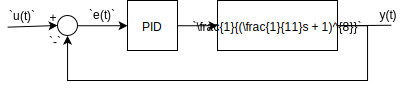
\includegraphics[width=0.9\textwidth]{img/schemat.png}
			\caption{\small{Schemat budowy przetwornika masy i siły oraz układ wyprowadzeń}}
		\end{figure}  \noindent
		Poszczególne parametry są dane następująco:
		\begin{center}
			\begin{tabular}{cc}
				$k$ (stała tensometrów) & 1,97 \\ 
				$b$ & 0,0193 m \\ 
				$l_1$ & 0,117 m \\ 
				$l_2$ & 0,112 m \\ 
				$h$ & $0,99 \cdot 10^{-3}$ m \\ 
				$E$ (moduł Younga) & $2.1 \cdot 10^{11} \, \mathrm{N/m^2}$ \\ 
				$\nu$ (liczba Poissona) & 0,3
			\end{tabular} 
		\end{center}
		
		\subsection{Pomiar masy lub siły metodą mostka niezrównoważonego}
			W tej części laboratorium mieliśmy za zadanie wyznaczyć czułości dla trzech różnych konfiguracji mostka. Czułość jest zadana wzorem:
			$$
				S_{CZ} = \frac{\Delta U_0 / U_z}{m}
			$$
			gdzie $\Delta U_0 / U_z$ to niezrównoważenie mostka, a $m$ to ważona masa. Względny błąd graniczny dany jest wzorem:
			$$
				\delta_{gr} = \frac{\Delta_{gr} \cdot 100\%}{S_{CZ}} 
			$$
			Postanowiliśmy wyznaczyć do przy pomocy metody różniczki zupełnej:
			$$
				\delta_{gr}= \frac{100\%}{S_{CZ}} 
				\cdot 
				\left(
					\left|\frac{\partial S_{CZ}}{\partial h} \Delta h\right|
					+
					\left|\frac{\partial S_{CZ}}{\partial l_1} \Delta l_1\right|
					+
					\left|\frac{\partial S_{CZ}}{\partial l_2} \Delta l_2\right|
					+
					\left|\frac{\partial S_{CZ}}{\partial b} \Delta b\right|
					+
					\left|\frac{\partial S_{CZ}}{\partial E} \Delta E\right|
					+
					\left|\frac{\partial S_{CZ}}{\partial \nu} \Delta \nu\right|
				\right)
			$$
			\subsubsection{konfiguracja pół-mostka z tensometrami wzdłużnymi}
				Czułość:
				$$
					S_{CZ} = \frac{3kgl_1}{Ebh^2} = 1,708 \cdot 10^{-3} \mathrm{\frac{mV/V}{kg}}
				$$
				Względny błąd graniczny:
				$$
					\delta_{gr} \approx 12,9\%
				$$
			\subsubsection{konfiguracja pół-mostka z tensometrem wzdłużnym i poprzecznym}
				Czułość:
				$$
					S_{CZ} = \frac{3kg(l_1 + \nu l_2)}{2Ebh^2} = 1,099 \cdot 10^{-3} \mathrm{\frac{mV/V}{kg}}
				$$
				Względny błąd graniczny:
				$$
					\delta_{gr} \approx 13,6\%
				$$
			\subsubsection{konfiguracja pełnego mostka z tensometrami wzdłużnymi i poprzecznymi}
				Czułość:
				$$
					S_{CZ} = \frac{3kg(l_1 + \nu l_2)}{Ebh^2} = 2,198 \cdot 10^{-3} \mathrm{\frac{mV/V}{kg}}
				$$
				Względny błąd graniczny:
				$$
				\delta_{gr} \approx 13,6 \%
				$$
		\subsection{Skalowanie torów pomiarowych w oparciu o obliczone teoretyczne czułości}
			Wartość czułości toru pomiarowego zadana jest wzorem:
			$$
				S = S_{CZ} S_W = S_{CZ} \cdot \frac{M_{skal}\alpha_{skal}}{(\Delta U_0 / U_Z)_{skal}}
			$$
			Wzmacniacz będzie wskazywać masę w sytuacji kiedy $S = 1$. Ponieważ postanowiliśmy dokonywać pomiarów z dokładnością do dwóch miejsc po przecinku w zakresie do 200 gramów musieliśmy przyjąć, że:
			\begin{center}
				\begin{tabular}{ccc}
					$\alpha_{skal}$ & = & 0,01 \\ 
					$M_{skal}$ & = & 20 000
				\end{tabular} 
			\end{center}
			W ten sposób iloczyn $M_{skal}\alpha_{skal}$ aby był równy 200 g. Wzór na rozrównoważenie mostka otrzymujemy przy tych założeniach jako następujący:
			$$
				\frac{\Delta U_0}{U_z} = M_{skal}\alpha_{skal} S_{CZ}
			$$
			Dla poszczególnych konfiguracji mostka przyjmuje to następujące wartości:
			\begin{center}
				\captionof{table}{\small{Niezrównoważenie mostka dla poszczególnych konfiguracji}}
				\begin{tabular}{|c|c|}
					\hline
					Konfiguracja & $(\Delta U_0 / U_z)_{skal}$ \\ \hline
					pół-mostek z tensometrami wzdłużnymi & 0,34153 \\ \hline  
					pół-mostek z tensometrem wzdłużnym i poprzecznym & 0,2198 \\ \hline 
					pełny mostek z tensometrem wzdłużnym i poprzecznym & 0,43961 \\ \hline
				\end{tabular}
			\end{center}
			W tym podpunkcie wybraliśmy konfigurację pół-mostka z tensometrami wzdłużnymi, gdyż ta znajdowała nie była ani największa, ani najmniejsza z trójki. Przystąpiliśmy więc do konfiguracji wzmacniacza pomiarowego dla tej wartości. 
			\\ \\
			Po skonfigurowaniu wzmacniacza pomiarowego przystąpiliśmy do weryfikacji poprawności dokonanych przez nas wyliczeń. Jednak przy pierwszym pomiarze dokonanym na 100 g wzorcu masy okazało się, że tor pomiarowy wyskalowany według wyznaczonych przez nas wartości wskazuje wartość inną niż waga ciężarka -- myli się o kilkanaście procent. Wynika to z tego, że mamy do czynienia z propagacją niepewności z jaką wyznaczyliśmy czułość czujnika masy.
		\subsection{Skalowanie torów pomiarowych w oparciu o wzorzec masy}
			Przystąpiliśmy więc do najczęściej stosowanej metody skalowania torów pomiarowych służących do pomiarów masy. Metoda ta w przypadku mostka tensometrycznego polega na ustawieniu wzmacniacza pomiarowego tak aby wskazywał rozrównoważenie mostka. Następnie odczytywaliśmy ją dla różnych mas wzorcowych. 
			\begin{center}
				\captionof{table}{\small{Niezrównoważenie mostka dla poszczególnych mas wzorcowych}}
				\begin{tabular}{|c|c|}\hline
					Masa wzorcowa & Wartość rozrównoważenia mostka mV/V \\ \hline
					10 g & 0,0193 \\ \hline
					20 g & 0,03866 \\ \hline
					50 g & 0,097 \\ \hline
					70 g & 0,13564 \\ \hline
					75 g & 0,1451 \\ \hline
					100 g & 0,1938 \\ \hline
				\end{tabular} 
			\end{center}
			Ponieważ mamy tu do czynienia z zależnością liniową, to do wyznaczenia czułości posłużyliśmy się regresją liniową, dopasowując prostą $y = ax$ do danych metodą najmniejszych kwadratów. Otrzymaliśmy w ten sposób współczynnik kierunkowy prostej równy $1,9378 \cdot 10^{-3} \mathrm{\frac{mV/V}{g}}$ -- jest to poszukiwana czułość czujnika.
			\newline 
			\newline 
			Wyznaczyliśmy na podstawie tej wartości rozrównoważenie jakie powinniśmy ustawić we wzmacniaczu pomiarowym aby otrzymać zamierzony zakres pomiarowy:
			$$
				(\Delta U_0 / U_z)_{skal} = 0,38756 \mathrm{\frac{mV}{V}}
			$$
			Po ustawieniu tej wartości masa była wskazywana poprawnie.
			\begin{figure}[H]
				\centering
				\includegraphics[width=0.8\textwidth]{img/wykresik.png}
				\caption{\small{Zależność rozrównoważenia mostka od masy}}
			\end{figure}  \noindent
		\subsection{Konfigurowanie torów pomiarowych w oparciu o oprogramowanie Catman\textregistered\ Express}
			Ostatnim celem laboratorium jaki udało nam się zrealizować było zapoznanie się z funkcjonalnością oprogramowania Catman\textregistered\ Express. Dowiedzieliśmy się przy tym jak można w prostszy i przyjaźniejszy użytkownikowi sposób skonfigurować wzmacniacz pomiarowy.
	\section{Wnioski i podsumowanie}
		Ćwiczenie te pozwoliło nam na wyznaczenie czułości poszczególnych mostków tensometrycznych oraz zapoznanie się ze skalowaniem ich parametrów tak aby pozwoliły nam w połączeniu ze wzmacniaczem pomiarowym MVD555 na skonstruowanie wagi. Po skonfigurowaniu wzmacniacza okazało się jednak, że pomiary znacznie odstają od wagi wzorców masy. Jak się okazuje jest to wynikiem propagacji błędów pomiarowych z pomiarów jakie zostały nam podane w treści zadania.
		\\
		\\
		Zdecydowanie nieprzyjazny użytkownikowi interfejs użytkownika z jakim zetknęliśmy się w przypadku wzmacniacza pomiarowego -- strasznie dużo operacji potrzebnych dla ustawienia jednego parametru -- mogliśmy w kolejnym kroku ćwiczenia zastąpić oprogramowaniem Catman\textregistered Express. Pierwsza z metod wymagała od nas wielokrotnego powtarzania jednej czynności i w przypadku chwili nieuwagi należało wykonać całą operację od nowa. 
\end{document}